
% Template for PLoS
% Version 3.1 February 2015
%
% To compile to pdf, run:
% latex plos.template
% bibtex plos.template
% latex plos.template
% latex plos.template
% dvipdf plos.template
%
% % % % % % % % % % % % % % % % % % % % % %
%
% -- IMPORTANT NOTE
%
% This template contains comments intended 
% to minimize problems and delays during our production 
% process. Please follow the template instructions
% whenever possible.
%
% % % % % % % % % % 
% % % % % % % % % % % % % % 
%
% Once your paper is accepted for publication, 
% PLEASE REMOVE ALL TRACKED CHANGES in this file and leave only
% the final text of your manuscript.
%
% There are no restrictions on package use within the LaTeX files except that 
% no packages listed in the template may be deleted.
%
% Please do not include colors or graphics in the text.
%
% Please do not create a heading level below \subsection. For 3rd level headings, use \paragraph{}.
%
% % % % % % % % % % % % % % % % % % % % % % %
%
% -- FIGURES AND TABLES
%
% Please include tables/figure captions directly after the paragr 
%
% DO NOT INCLUDE GRAPHICS IN YOUR MANUSCRIPT
% - Figures should be uploaded separately from your manuscript file. 
% - Figures generated using LaTeX should be extracted and removed from the PDF before submission. 
% - Figures containing multiple panels/subfigures must be combined into one image file before submission.
% For figure citations, please use "Fig." instead of "Figure".
% See http://www.plosone.org/static/figureGuidelines for PLOS figure guidelines.
%
% Tables should be cell-based and may not contain:
% - tabs/spacing/line breaks within cells to alter layout or alignment
% - vertically-merged cells (no tabular environments within tabular environments, do not use \multirow)
% - colors, shading, or graphic objects
% See http://www.plosone.org/static/figureGuidelines#tables for table guidelines.
%
% For tables that exceed the width of the text column, use the adjustwidth environment as illustrated in the example table in text below.
%
% % % % % % % % % % % % % % % % % % % % % % % %
%
% -- EQUATIONS, MATH SYMBOLS, SUBSCRIPTS, AND SUPERSCRIPTS
%
% IMPORTANT
% Below are a few tips to help format your equations and other special characters according to our specifications. For more tips to help reduce the possibility of formatting errors during conversion, please see our LaTeX guidelines at http://www.plosone.org/static/latexGuidelines
%
% Please be sure to include all portions of an equation in the math environment.
%
% Do not include text that is not math in the math environment. For example, CO2 will be CO\textsubscript{2}.
%
% Please add line breaks to long display equations when possible in order to fit size of the column. 
%
% For inline equations, please do not include punctuation (commas, etc) within the math environment unless this is part of the equation.
%
% % % % % % % % % % % % % % % % % % % % % % % % 
%
% Please contact latex@plos.org with any questions.
%
% % % % % % % % % % % % % % % % % % % % % % % %

\documentclass[10pt,letterpaper]{article}
\usepackage[top=0.85in,left=2.75in,footskip=0.75in]{geometry}

% Use adjustwidth environment to exceed column width (see example table in text)
\usepackage{changepage}

% Use Unicode characters when possible
\usepackage[utf8]{inputenc}

% textcomp package and marvosym package for additional characters
\usepackage{textcomp,marvosym}

% fixltx2e package for \textsubscript
\usepackage{fixltx2e}

% amsmath and amssymb packages, useful for mathematical formulas and symbols
\usepackage{amsmath,amssymb}

% cite package, to clean up citations in the main text. Do not remove.
\usepackage{cite}

% Use nameref to cite supporting information files (see Supporting Information section for more info)
\usepackage{nameref,hyperref}

% line numbers
\usepackage[right]{lineno}

% ligatures disabled
\usepackage{microtype}
\DisableLigatures[f]{encoding = *, family = * }

% rotating package for sideways tables
\usepackage{rotating}

% Remove comment for double spacing
%\usepackage{setspace} 
%\doublespacing

\usepackage{amsmath}
\usepackage{graphicx}
\usepackage{rotating}
\usepackage{tikz}

% Text layout
\raggedright
\setlength{\parindent}{0.5cm}
\textwidth 5.25in 
\textheight 8.75in

% Bold the 'Figure #' in the caption and separate it from the title/caption with a period
% Captions will be left justified
\usepackage[aboveskip=1pt,labelfont=bf,labelsep=period,justification=raggedright,singlelinecheck=off]{caption}

% Use the PLoS provided BiBTeX style
\bibliographystyle{plos2015}

% Remove brackets from numbering in List of References
\makeatletter
\renewcommand{\@biblabel}[1]{\quad#1.}
\makeatother

% Leave date blank
\date{}

% Header and Footer with logo
\usepackage{lastpage,fancyhdr,graphicx}
\usepackage{epstopdf}
\pagestyle{myheadings}
\pagestyle{fancy}
\fancyhf{}
\lhead{\includegraphics[width=2.0in]{PLOS-submission.eps}}
\rfoot{\thepage/\pageref{LastPage}}
\renewcommand{\footrule}{\hrule height 2pt \vspace{2mm}}
\fancyheadoffset[L]{2.25in}
\fancyfootoffset[L]{2.25in}
\lfoot{\sf PLOS}

%% Include all macros below

\newcommand{\lorem}{{\bf LOREM}}
\newcommand{\ipsum}{{\bf IPSUM}}

%% END MACROS SECTION


\begin{document}
\vspace*{0.35in}

% Title must be 250 characters or less.
% Please capitalize all terms in the title except conjunctions, prepositions, and articles.
\begin{flushleft}
{\Large
\textbf\newline{Comparison of primary glioblastoma Single-cell and Tissue RNA-seq co-expression networks - Submission to PLOS Journals}
}
\newline
% Insert author names, affiliations and corresponding author email (do not include titles, positions, or degrees).
\\
Brian Arand\textsuperscript{2},
Raghu Machiraju\textsuperscript{1, 2},
Kun Huang\textsuperscript{1, 2}

\bigskip
\bf{1} Department of Biomedical Informatics, The Ohio State University, Columbus, Ohio, The United States of America
\\
\bf{2} Department of Computer Science and Engineering, The Ohio State University, Columbus, Ohio, The United States of America
\\
%\bf{3} Affiliation Dept/Program/Center, Institution Name, City, %State, Country
%\\
\bigskip

% Insert additional author notes using the symbols described below. Insert symbol callouts after author names as necessary.
% 
% Remove or comment out the author notes below if they aren't used.
%
% Primary Equal Contribution Note
%\Yinyang These authors contributed equally to this work.

% Additional Equal Contribution Note
% Also use this double-dagger symbol for special authorship notes, such as senior authorship.
%\ddag These authors also contributed equally to this work.

% Current address notes
%\textcurrency a Insert current address of first author with an address update
% \textcurrency b Insert current address of second author with an address update
% \textcurrency c Insert current address of third author with an address update

% Deceased author note
%\dag Deceased

% Group/Consortium Author Note
%\textpilcrow Membership list can be found in the Acknowledgments section.

% Use the asterisk to denote corresponding authorship and provide email address in note below.
%* CorrespondingAuthor@institute.edu

\end{flushleft}
% Please keep the abstract below 300 words
\section*{Abstract}

% Please keep the Author Summary between 150 and 200 words
% Use first person. PLOS ONE authors please skip this step. 
% Author Summary not valid for PLOS ONE submissions.   
%\section*{Author Summary}
%Lorem ipsum dolor sit amet, consectetur adipiscing elit. Curabitur eget porta erat. Morbi consectetur est vel gravida pretium. Suspendisse ut dui eu ante cursus gravida non sed sem. Nullam sapien tellus, commodo id velit id, eleifend volutpat quam. Phasellus mauris velit, dapibus finibus elementum vel, pulvinar non tellus. Nunc pellentesque pretium diam, quis maximus dolor faucibus id. Nunc convallis sodales ante, ut ullamcorper est egestas vitae. Nam sit amet enim ultrices, ultrices elit pulvinar, volutpat risus.

\linenumbers

\section*{Introduction}
The isolation of individual cells’ transcriptome profiles has been largely a theoretical concept to bioinformaticians. And accordingly, transcriptomic inquiry has been limited to those questions regarding tissues, potentially composed of a heterogeneous hodgepodge of cellular types, subtypes, and states. But with the advent of Single-Cell RNA sequencing (RNASeq) technology, comes the potential for refined resolution in transcriptomic datasets. And expectedly, recent publications suggest a peaking interest in this new landscape of informatics. It has been shown that many bioinformatics techniques that were developed for bulk-cell tissue samples can be effectively applied to single-cellular datasets. %REFERENCES HERE!!!!
However, co-expression network analysis has largely been an unexplored area of analysis in regards to single-cell RNASeq data. To fill this gap, we leverage this new technology to construct and analyze gene co-expression networks for primary glioblastoma single-cell samples. Glioblastoma is widely known to be a heterogeneous cancer, making it a prime candidate for single-cellular inquiries. For instance, we hypothesized that the averaging of single-cells’ profiles within a tissue sample may mask or otherwise confound downstream gene correlations based analysis. Correlation between two genes may exist across tissue samples purely due to changing proportion of cellular subtypes within those samples. However, a single-cellular perspective, of the same tumors may theoretically filter out those artificial tissue-level correlations. And so correlation based analyses, like co-expression network analysis, require study. In our work, we begin this journey by looking at network mining, module detection, and gene enrichment analysis at both the single-cell and bulk cell (tissue sample) levels. The final goal of this work is to shed light on the convoluted intricacies of inter-cellular genomic landscape of glioblastoma tissue from a single-cellular perspective.

% You may title this section "Methods" or "Models". 
% "Models" is not a valid title for PLoS ONE authors. However, PLoS ONE
% authors may use "Analysis" 
\section*{Materials and Methods}

\begin{figure}[h]
\centering
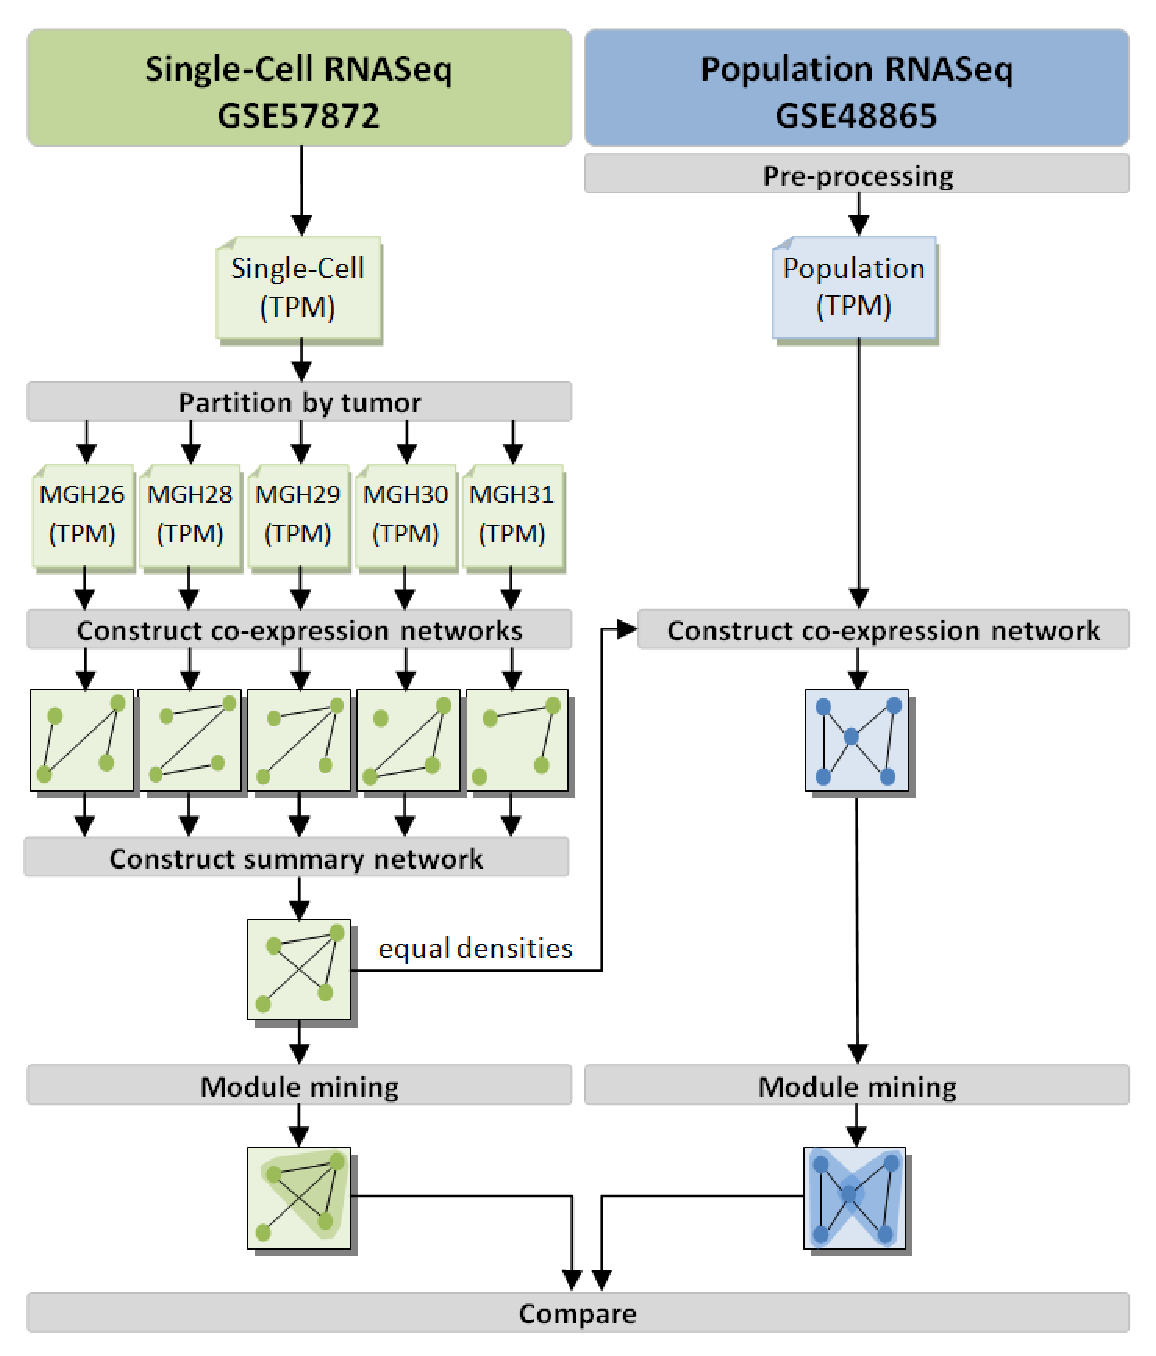
\includegraphics[width=80mm]{Figures/Workflow}
\caption{{\bf Network comparison workflow.} Note that there is no  partition nor aggregation step in the bulk RNASeq pipeline. Moreover, note that edges of the constructed bulk co-expression network are filtered to achieve the closest network density possible to that realized in the Single-Cell pipeline. }
\label{fig:workflow}
\end{figure}

\subsection*{Single-Cell Data}
\subsection*{Single-Cell RNASeq Samples }

\begin{figure}[t]
\centering
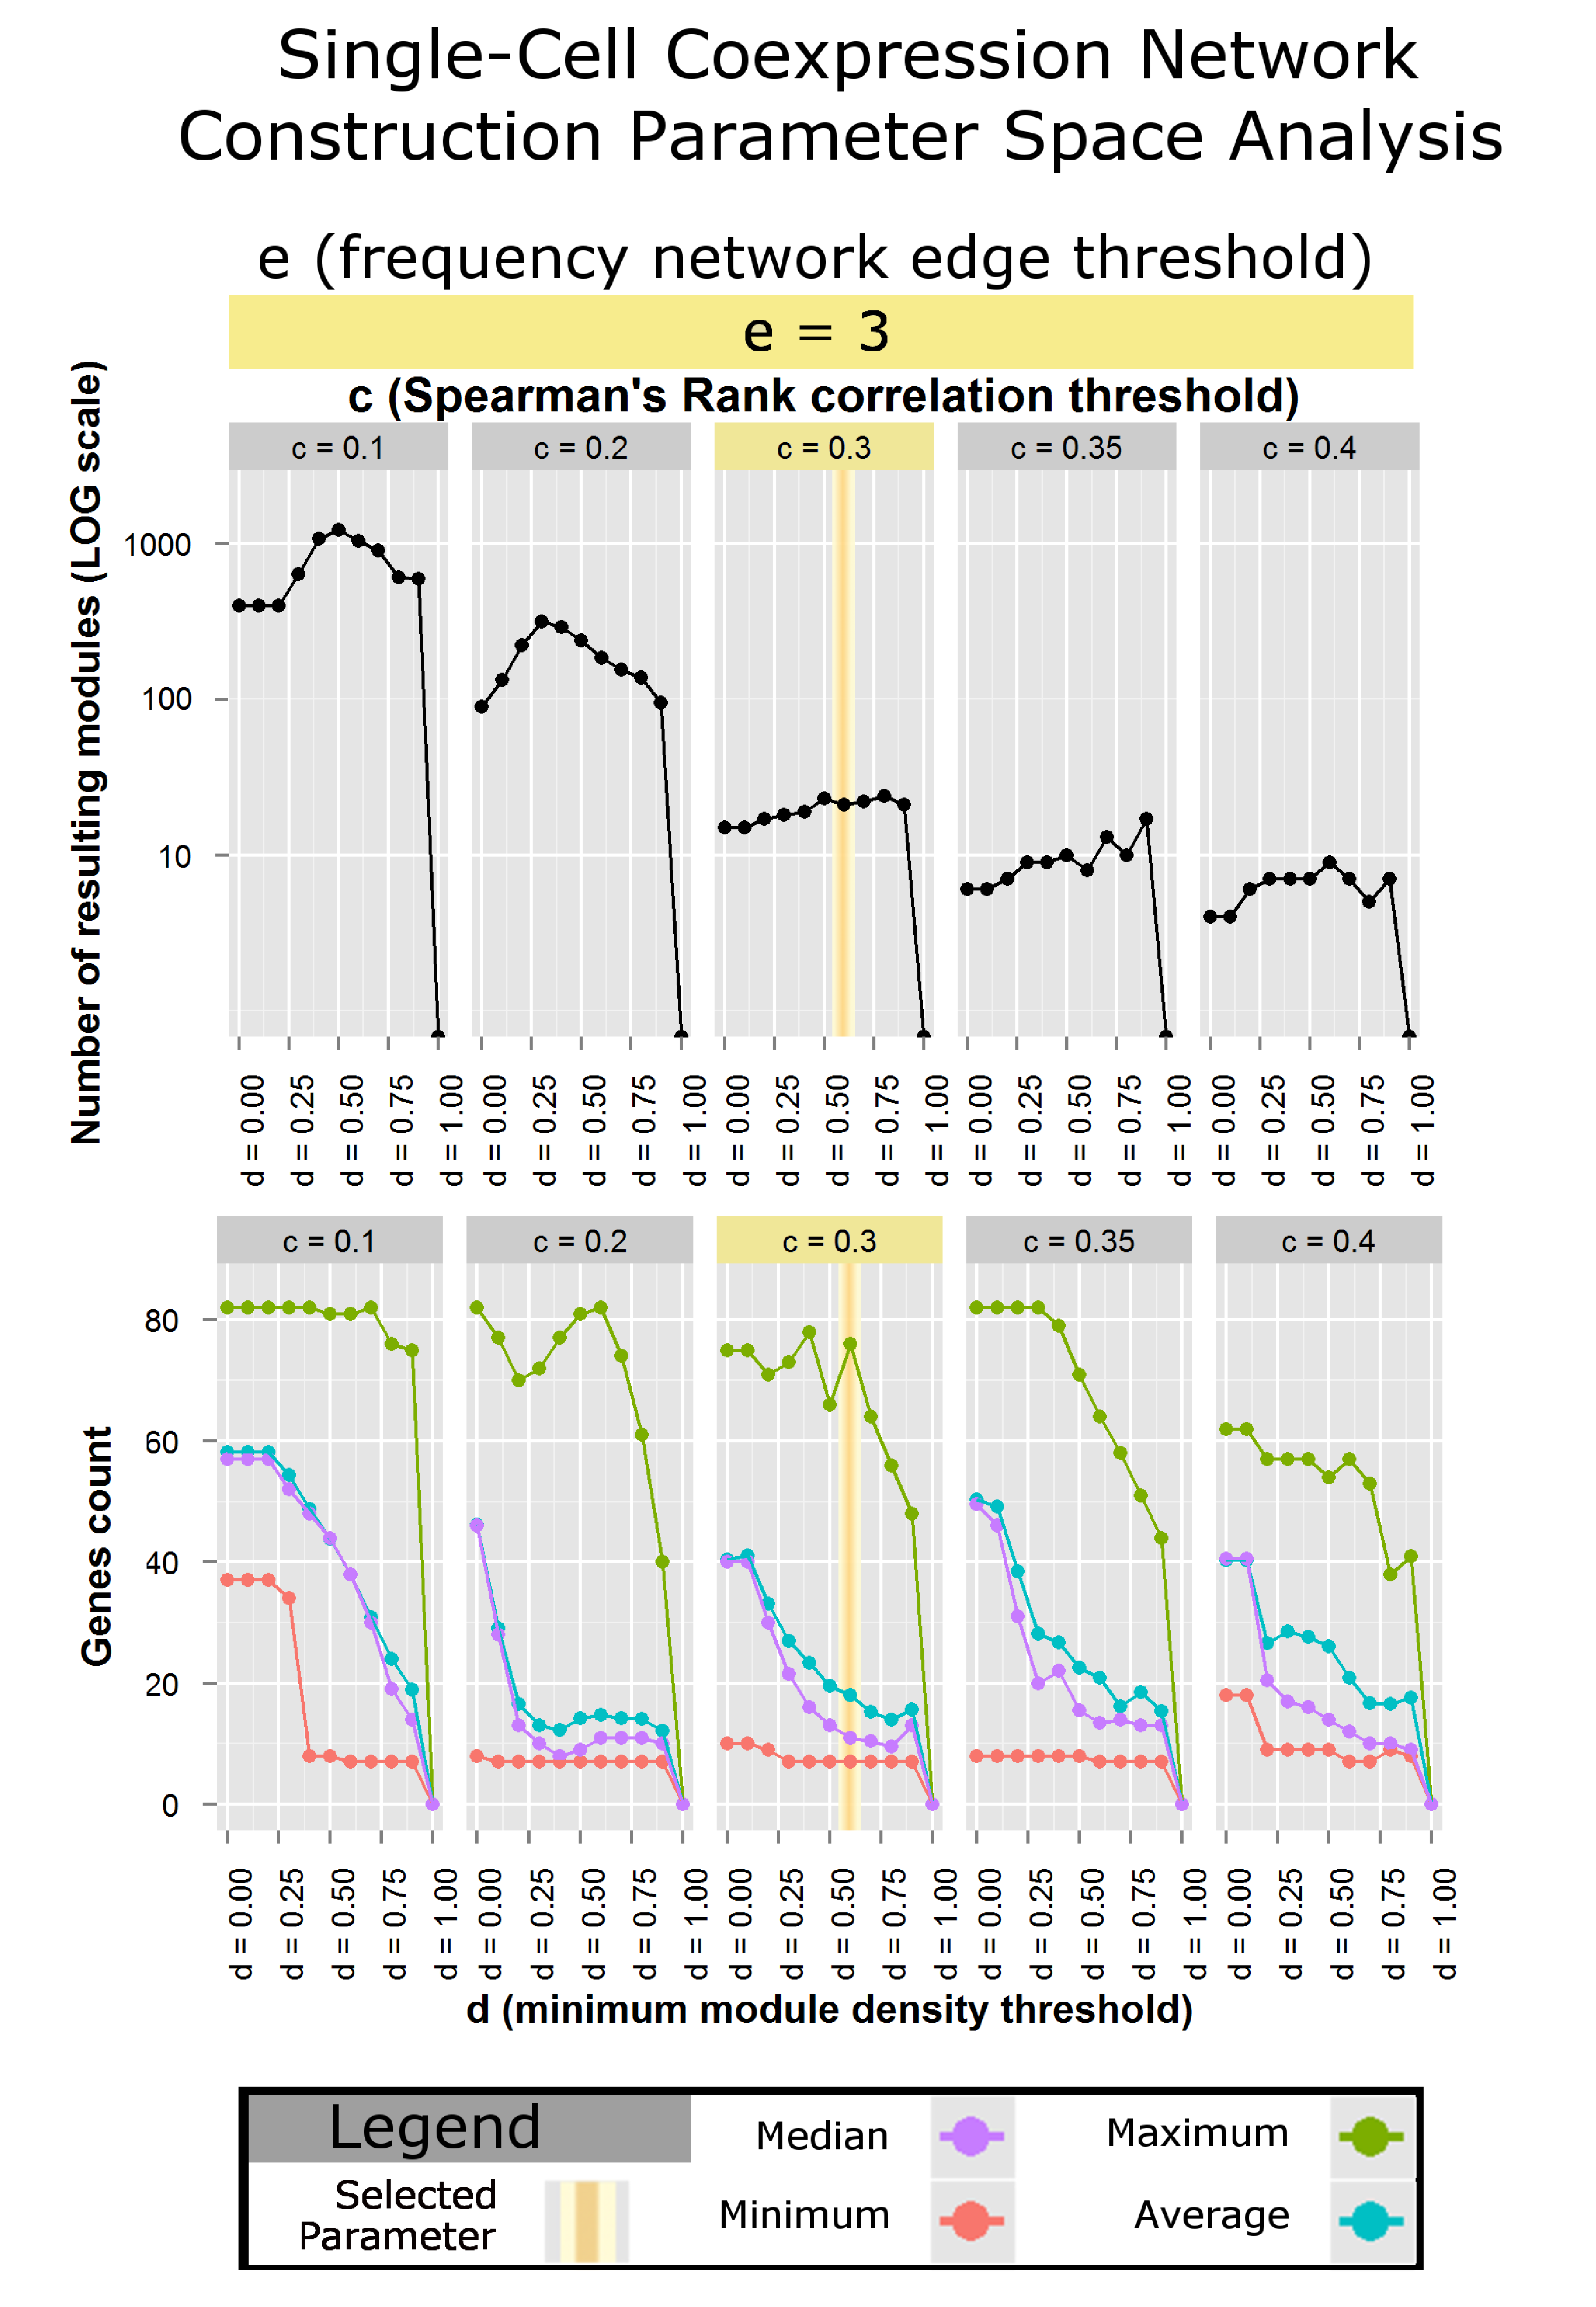
\includegraphics[width=80mm]{Figures/ParameterSpaceE=3}
\label{Parameter Space Figure}
\end{figure}

\begin{figure}[h]
\centering
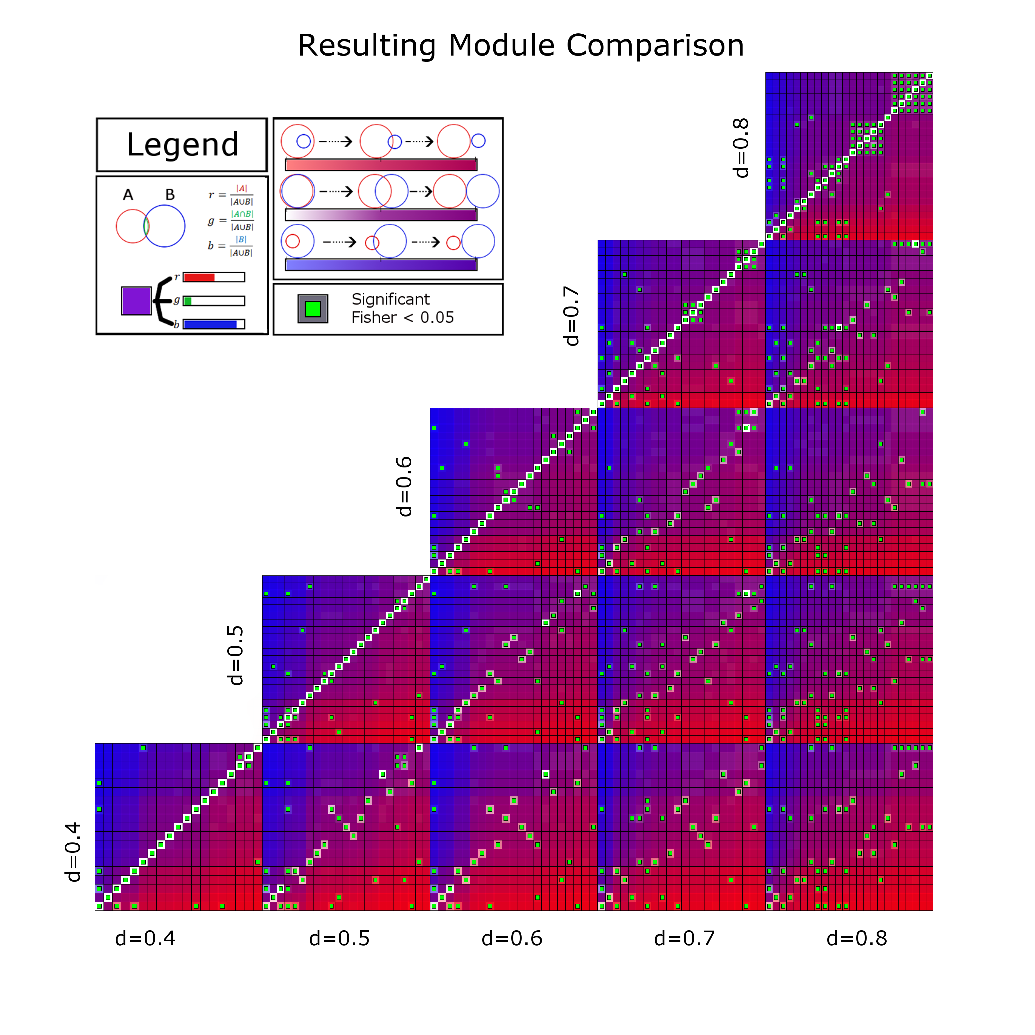
\includegraphics[width=100mm]{Figures/moduleStaryNight2}
\caption{\textbf{Parameterization space starry map.} Here we display the exhaustive gene-set by gene-set enrichment profiles for those modules output by 5 different runs of CODENSE for different values of the minimum density threshold $d$. The color of each square encodes the size of some gene set $A$, some gene set $B$, and the size of $A\cap{}B$ relative to $A\cup{}B$. These three values are encoded into the red, blue, and green channels of the square respectively. Thus, the whiter a square is the more similar $A$ and $B$ are. Furthermore, a Fisher's exact test was performed for significant enrichment per gene set pair. Placement of a small, green token indicates significant overlap between modules. 
\label{fig:starryNight1}
\end{figure}

\begin{equation}\label{equation1}
y_{i} = \frac{\sum_{s} \log_2(x_{si} + 1)} {N_t}
\end{equation}

\begin{equation}\label{equation2}
y_{si}=\sum_{s} \log_2(x_{si} + 1)-y_i
\end{equation}

\subsubsection{Network Construction}
In our analysis, single-cell samples were grouped by tumor of origin, $t$. For each group, a gene-by-gene Spearman’s rank correlation matrix was calculated as in Eq. \ref{equation3} .

\begin{equation}\label{equation3}
 P_t = \left[ \begin{array}{ccc}
\rho_{11t} & \ldots & \rho_{1kt} \\
\vdots & \ddots & \vdots \\
\rho_{k1t} & \ldots & \rho_{kkt}i \end{array} \right]
\end{equation}

Where $\rho_{ijt}$ is the Spearman’s correlation between the $i^{th}$ and $j^{th}$ gene of tumor $t$. Co-expression matrices were then created by filtering at the same Spearman’s rank threshold, $c$, to produce binary matrices, $B_t$, per tumor. 

\begin{equation}\label{equation4}
B_t = \left[ \begin{array}{ccc}
b_{11t} & \ldots & b_{1kt} \\
\vdots & \ddots & \vdots \\
b_{k1t} & \ldots & b_{kkt}i \end{array}
\right], b_{ijt}= \begin{cases} 
1, & \vert\rho_{ijt}\vert\ge c \\
0, & o.w. \\
\end{cases}
\end{equation}


The binary matrices were then aggregated into a single frequency matrix, $F$. This aggregation is performed in an attempt to attenuate patient-specific signals and focus, rather, on glioblastoma-specific patterns of gene co-expression.

\begin{equation}\label{equation5}
F = \left[ \begin{array}{ccc}
\vdots & \ddots & \vdots \\
\end{equation}

\subsubsection{Module Detection}
It is this matrix $F$ that is fed into the CODENSE software to be converted into a summary network, $S$, and then mined for high-density modules \cite{Hu2005}.  

\begin{equation}\label{equation6}
S=(V,E), \text{ where } v_i,v_j \in V \text{ and } (v_i,v_j) \in E \leftrightarrow f_{ij} \ge e
\end{equation}
Frequency threshold threshold $e$ was set to be 3 meaning that in order for a given'



\subsection{Bulk Cell Samples}
Our bulk cell sample control comes from GEO accession GSE48865. 274 glioma tissue samples make up this dataset, of which, 59 were identified as primary, stage-4 glioblastoma tissue samples. We filtered out any reads from the 59 samples with more than 10\% of its nucleotides designated as unknown bases, and any read with more than 50\% of its bases having Sanger phred+33 quality scores less than 5. After filtering, we retained 1,388,064,773 reads in total. 

Each filtered sample was then aligned to hg19 transcriptome (GRCh37) using bow-tie (version 1.1.1 with default parameters provided by RSEM) and TPM values per gene were estimated using RSEM (version 1.2.3). 73\% of the reads were aligned successfully either uniquely or multi-mapped. 

%\begin{figure}[h]
%\centering
%\includegraphics[width=80mm]{{Figures/GeneMembershipProfile}}
%\caption{\textbf{Sample gene profile.}}
%\label{fig:profile}
%\end{figure}

\subsubsection{Network Construction and Module Detection}


Modules were also found using the CODENSE algorithm using the same parameterization used in the single-cell workflow described above.

\subsection{Enrichment}


% Results and Discussion can be combined.
\section*{Results}


\begin{figure}[h]
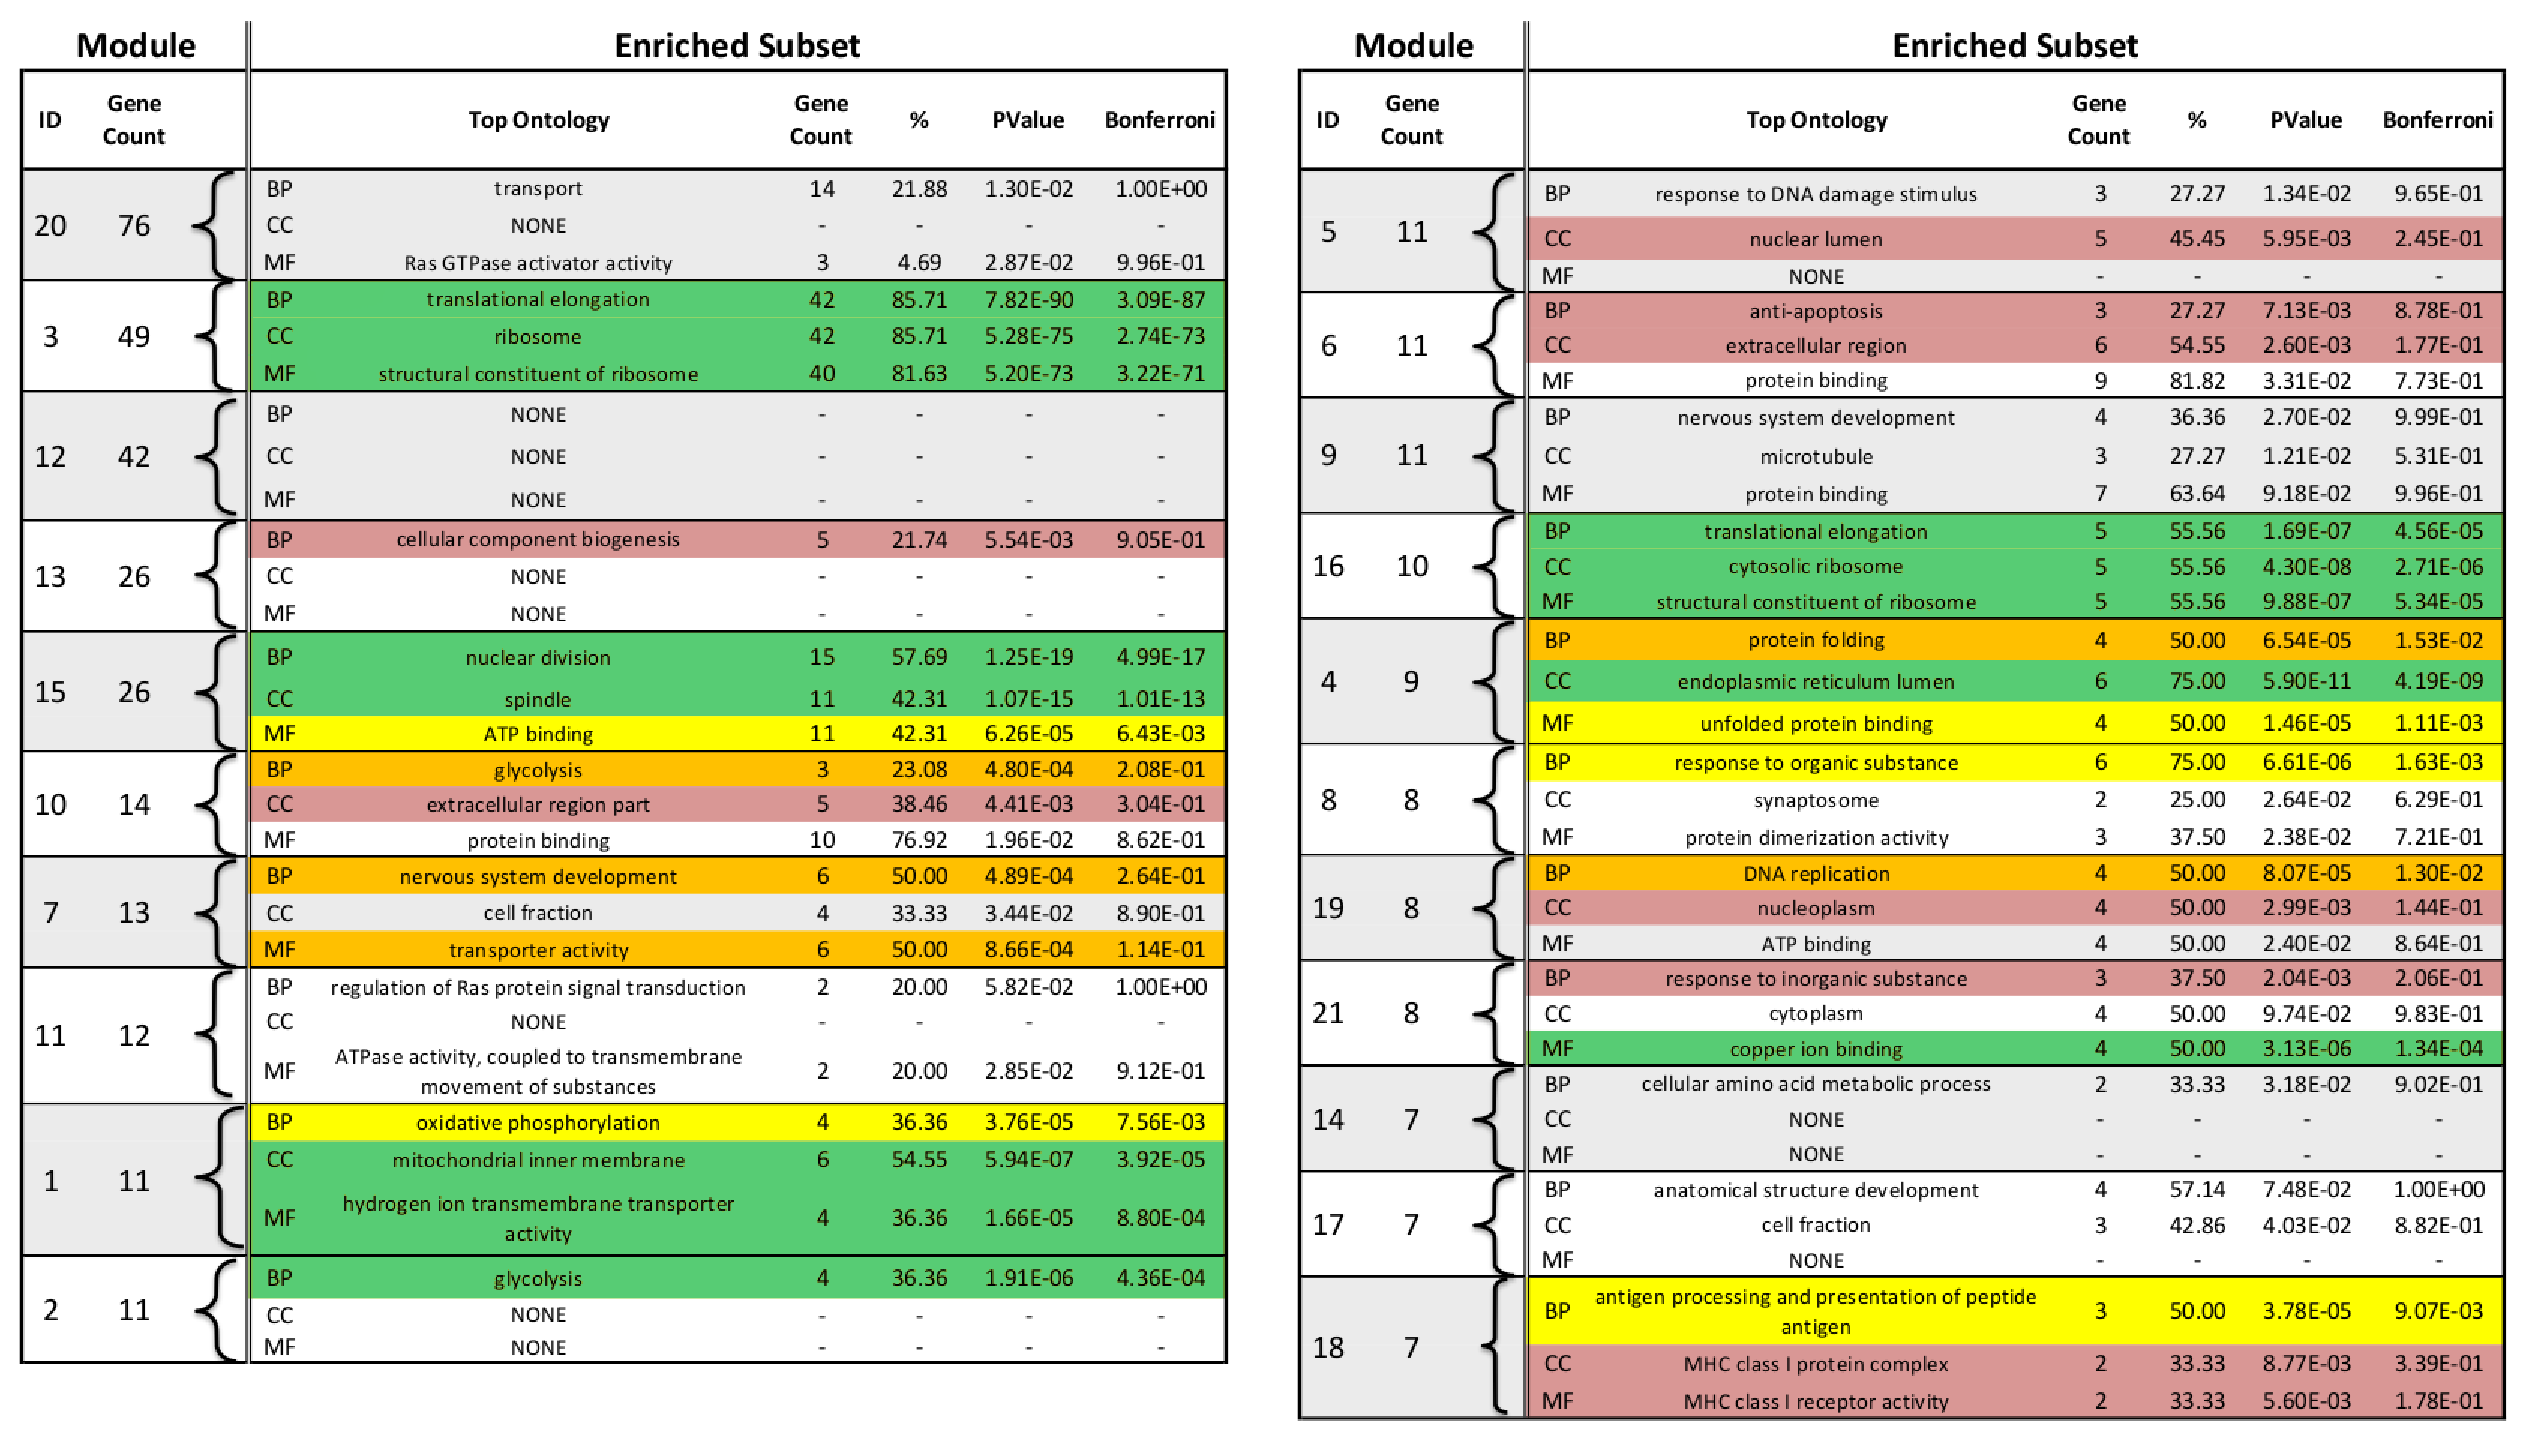
\includegraphics[width=120mm]{{Figures/toDavidGSE57872_freqNet_03_clusters}}
\caption{\textbf{Single-cell network module ontology enrichment.} A list of the modules output from the CODENSE algorithm ordered by module size, each enriched for BP, CC, and MC ontologies. Row color denotes a certain statistical significance as demarcated in the figure legend.}%
\label{fig:57872Clusts}
\end{figure}

\begin{figure}[h]
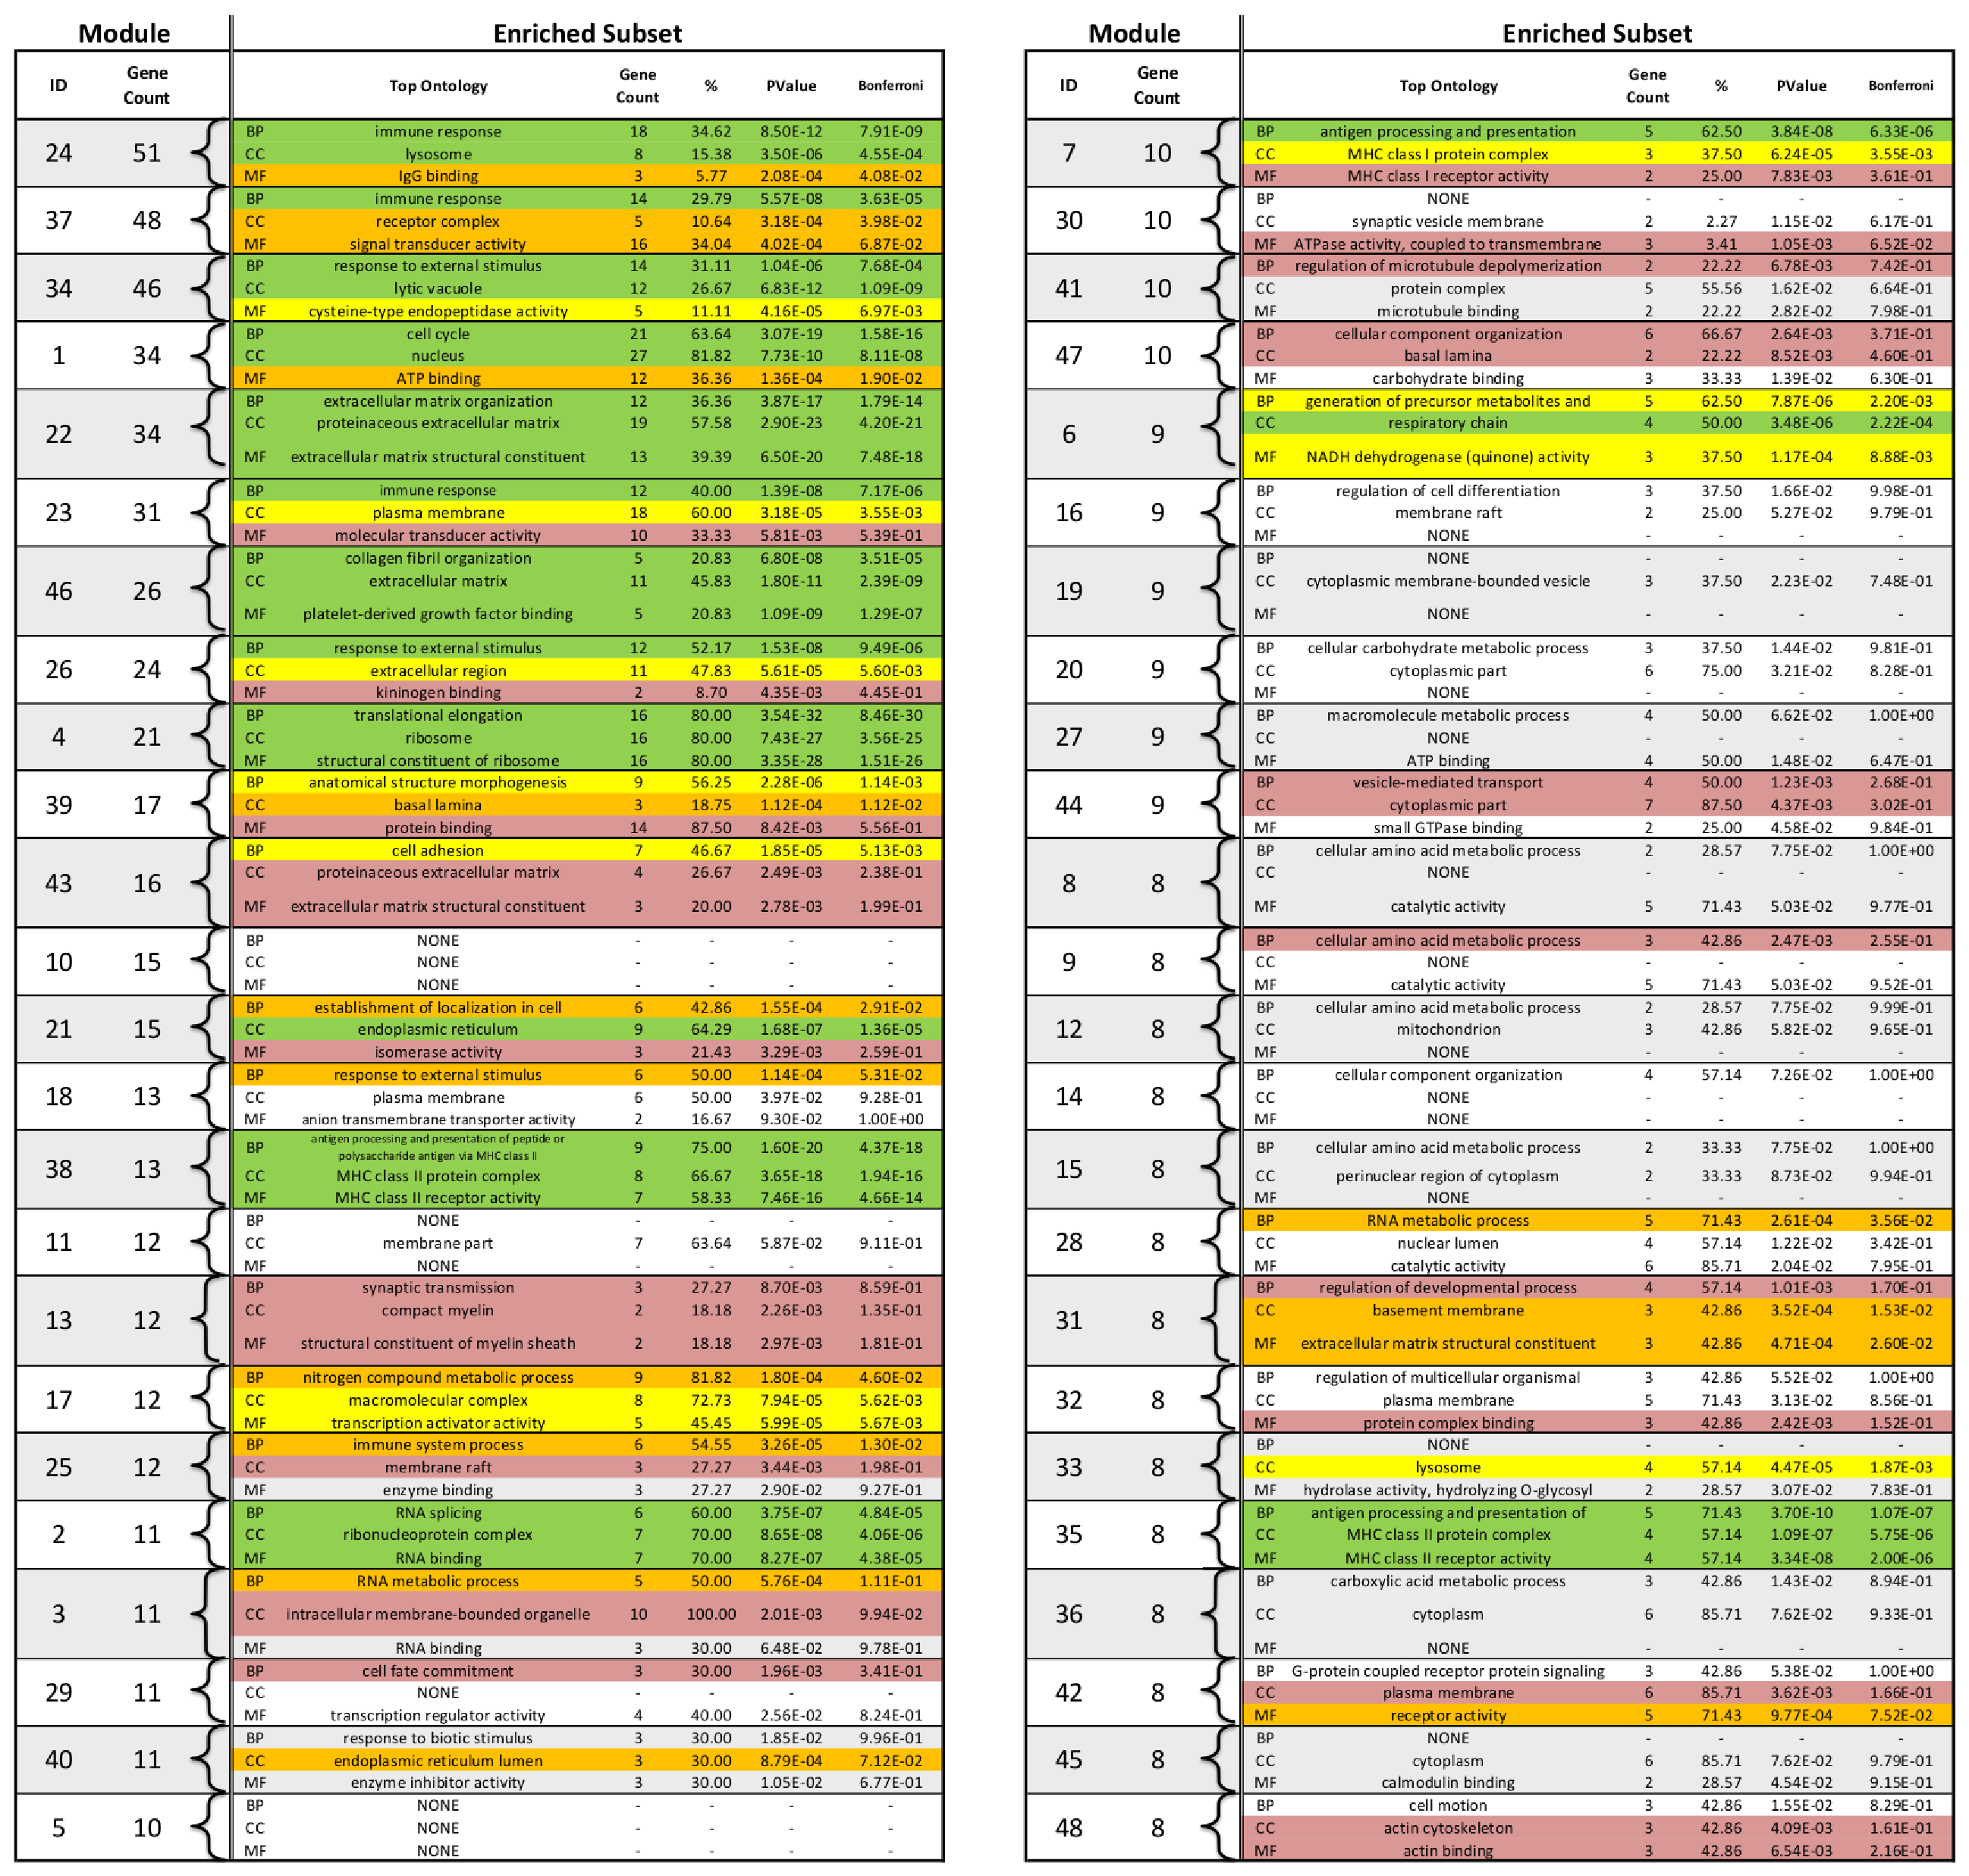
\includegraphics[width=120mm]{{Figures/toDavidGSE48865_filt_0002_clusters}}
\label{fig:48865Clusts}
\end{figure}


Make note that one of the most significantly enriched ontolodies reported for the bulk modules was extracellular matrix organization. Single-cell modules did not enrich for this specific ontology. 


\begin{sidewaysfigure}[h]
\centering
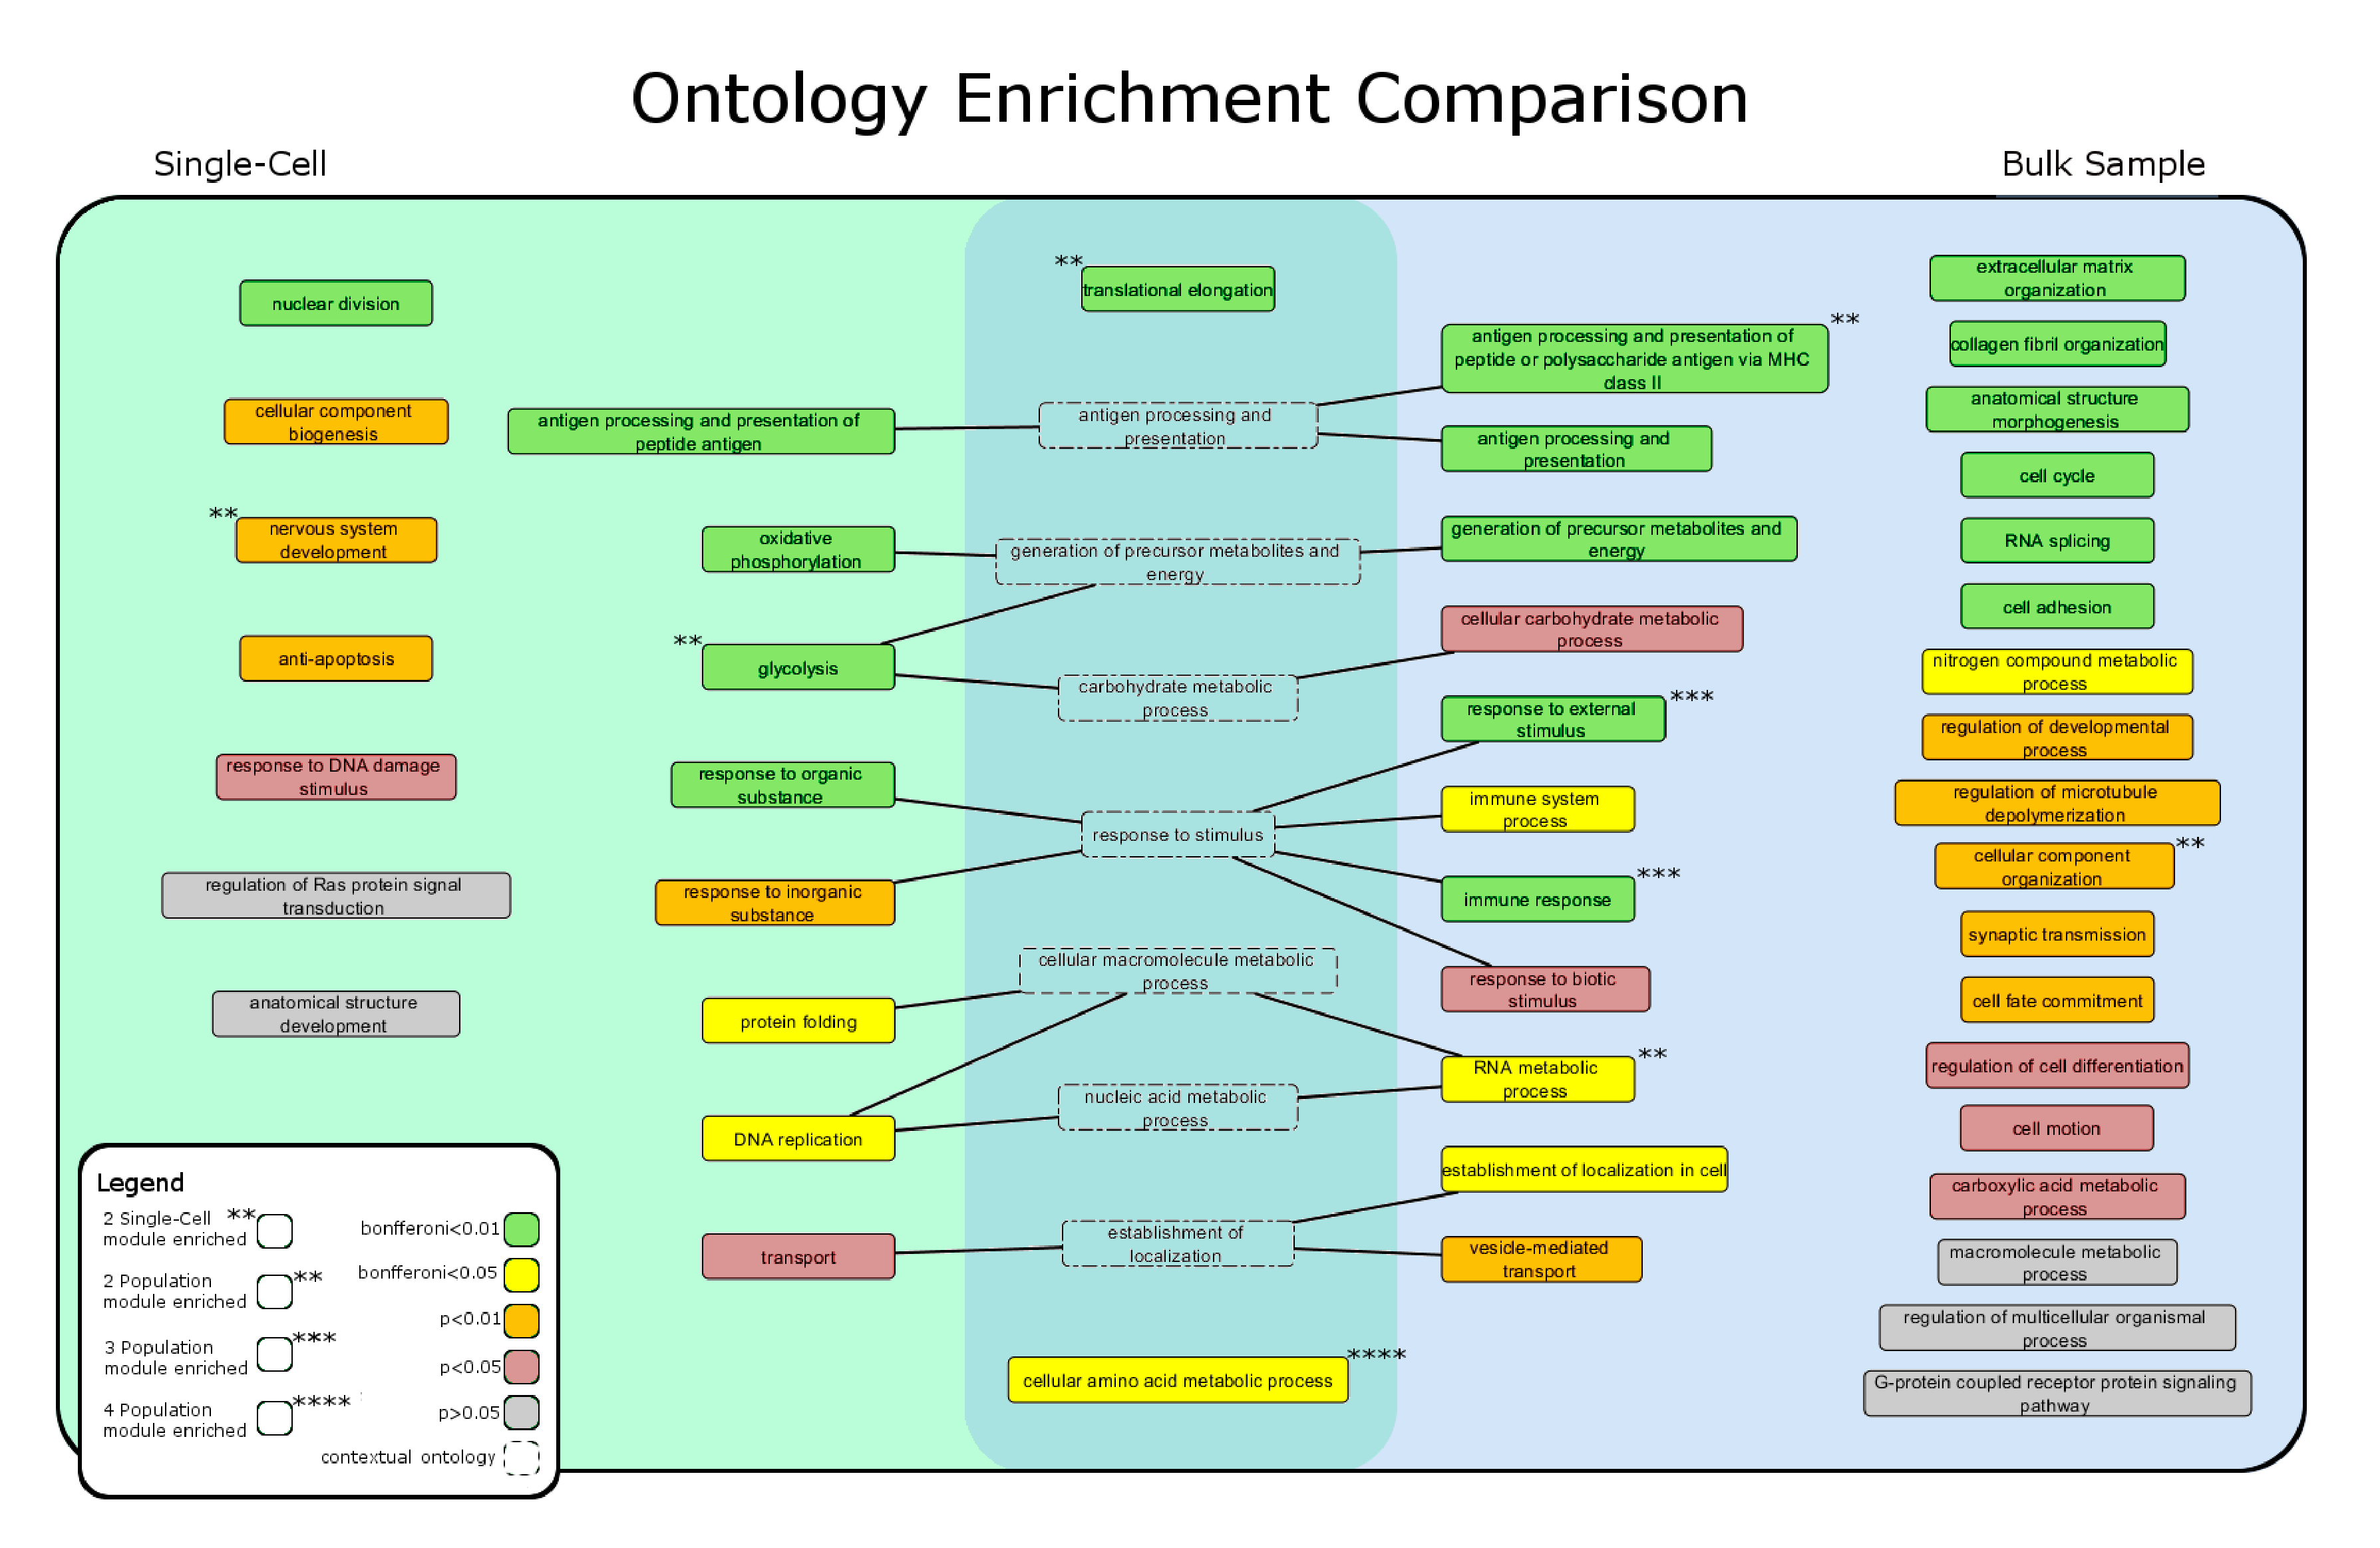
\includegraphics[width=180mm]{Figures/PopVsSCToCytoscape}
\label{fig:venn}
\end{sidewaysfigure}

A gene-level comparison of the resulting modules of the two data sets is also provided in fig. \ref{fig:starryMap2}. We find 3 or 4 groups of modules within the bulk output that are co-enriched for each other. Meaning that a given subgroup of modules share a significant number of genes with each other. We hypothesis that this co-enrichment occurred as a result of the specific parameterization used to construct and mine the network for modules. By either raising the correlation threshold, $c$, or raising the minimum module density threshold, $d$, these co-enriched modules may fuse into a larger module. We further hypothesis, by taking cues from the ontology enrichment of the co-enriched modules, that the resulting larger modules would likely enrich for immune response, metabolic processes, and extracellular matrix ontologies. 


\begin{figure}[h]
\centering
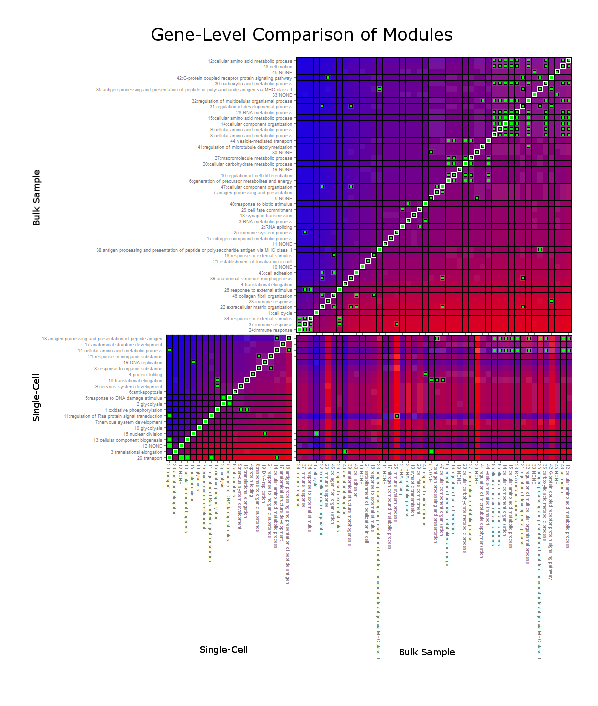
\includegraphics[width=125mm]{Figures/moduleCompareStaryMap2}
\label{fig:starryMap2}
\end{figure}

\begin{sidewaysfigure}[h]
\centering
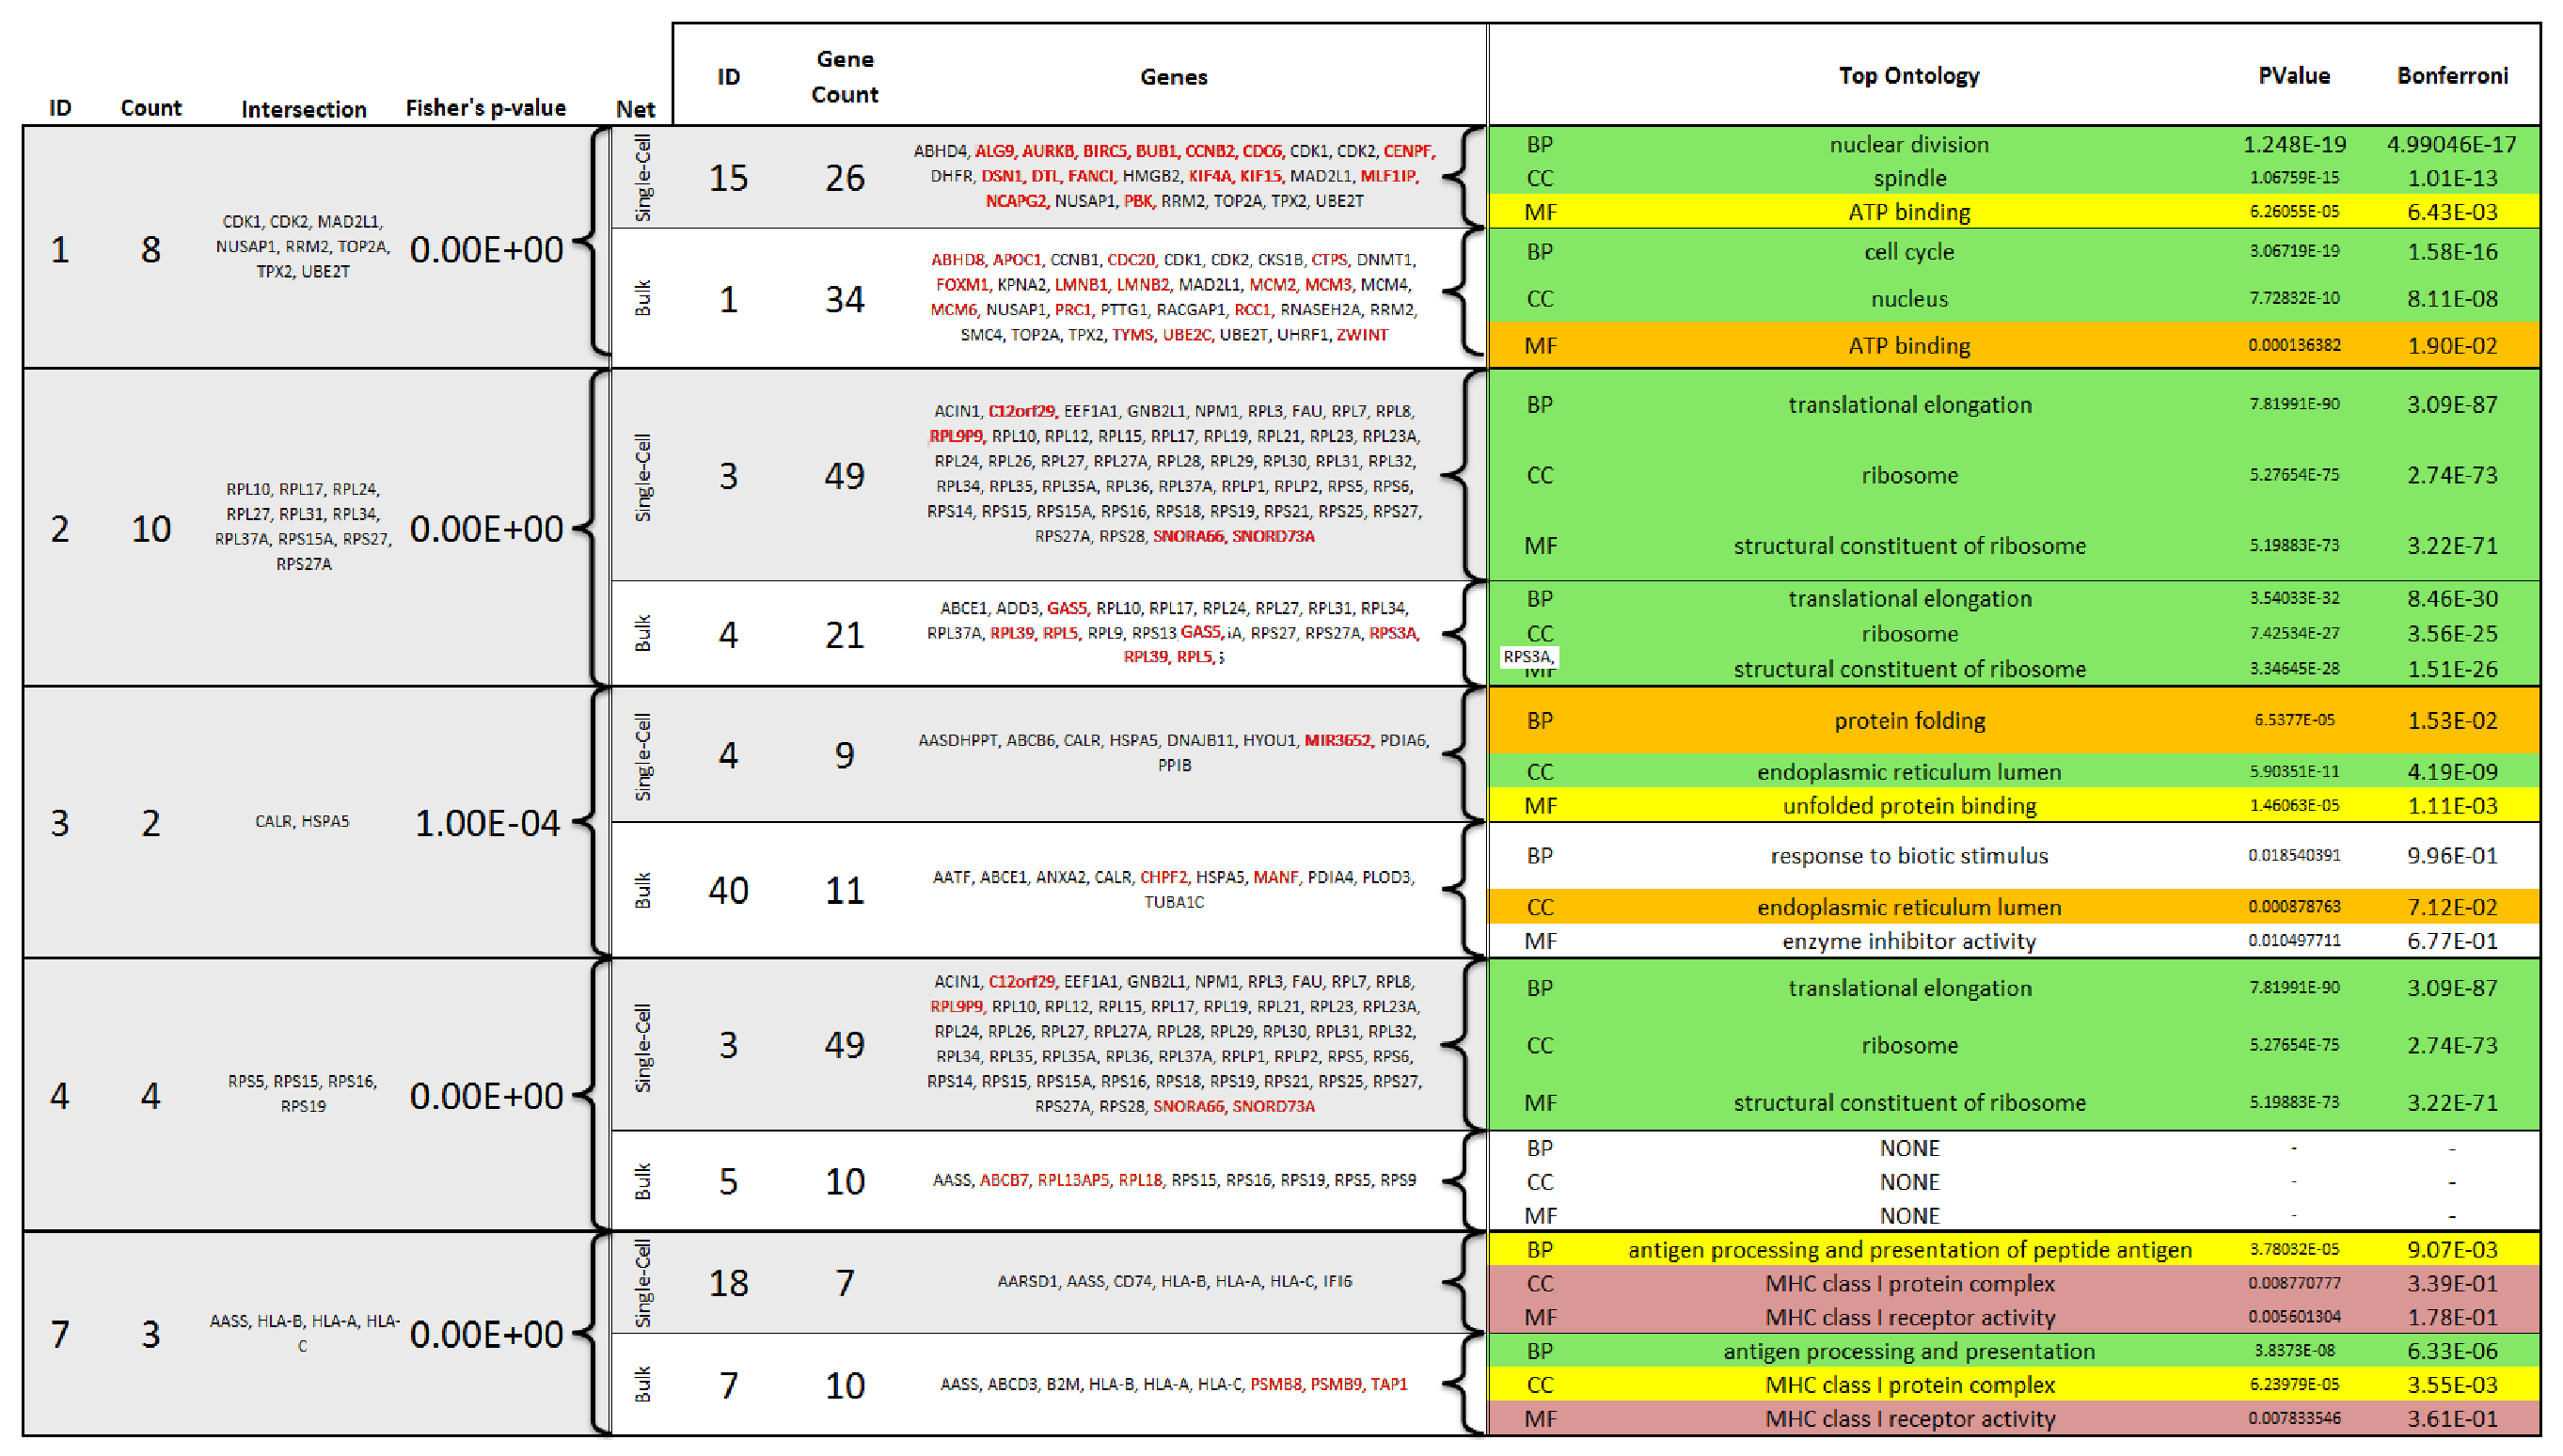
\includegraphics[width=180mm]{Figures/PopVsSCGeneLevel}
\label{fig:geneLevelChart}
\end{sidewaysfigure}

\clearpage 

\section*{Discussion}

Our analysis illustrates the potential of single-cell co-expression network module enrichment analysis as a potential tool for biological inquiry. We find that, when taking the contextual approach to comparing the sets of reported ontologies, most of the more significantly enriched ontologies reported by the bulk data were related to those reported by single-celled data. Furthermore, when taking a more refined, gene-level approach to this comparison a handful of modules are still in agreement.


Further comparisons and contrast may indeed be possible. Conservative filtering in the single-celled pipline may be limiting the results in this work. Accounting for noise in single-celled data could strengthen the claims possible in co-expression module enrichment comparisons in the future. 

\nolinenumbers

%\section*{References}
% Either type in your references using

% \begin{thebibliography}{}
% \bibitem{}
% Text
% \end{thebibliography}
%
% OR
%
% Compile your BiBTeX database using our plos2015.bst
% style file and paste the contents of your .bbl file
% here.
% 
%\begin{thebibliography}{10}
%\bibitem{bib1}
%Devaraju P, Gulati R, Antony PT, Mithun CB, Negi VS. Susceptibility to SLE in South Indian Tamils may be influenced by genetic selection pressure on TLR2 and TLR9 genes. Mol Immunol. 2014 Nov 22. pii: S0161-5890(14)00313-7. doi: 10.1016/j.molimm.2014.11.005

%\bibitem{bib2}
%Huynen MMTE, Martens P, Hilderlink HBM. The health impacts of globalisation: a conceptual framework. Global Health. 2005;1: 14. Available: http://www.globalizationandhealth.com/content/1/1/14.

%\end{thebibliography}
\bibliographystyle{plainnat}
\bibliography{References}

\end{document}

